\chapter{MACHINE LEARNING MODEL DEVELOPMENT}

\section{Workflow and System Architecture}

Figure~\ref{fig:workflow} shows the pipeline that produced every number in this
report. It is implemented as importable modules under \texttt{src/} rather than as
a single notebook, so that the notebooks, the tests and the report generator all
call the same code. The three columns correspond to the three partitions of the
data: preparation, learning and assessment. The horizontal connectors mark the
only points at which data moves between them, which is what makes the leakage
argument in Section~4.4 checkable: the test partition is not reachable from the
learning column.

\begin{figure}[htbp]
\centering
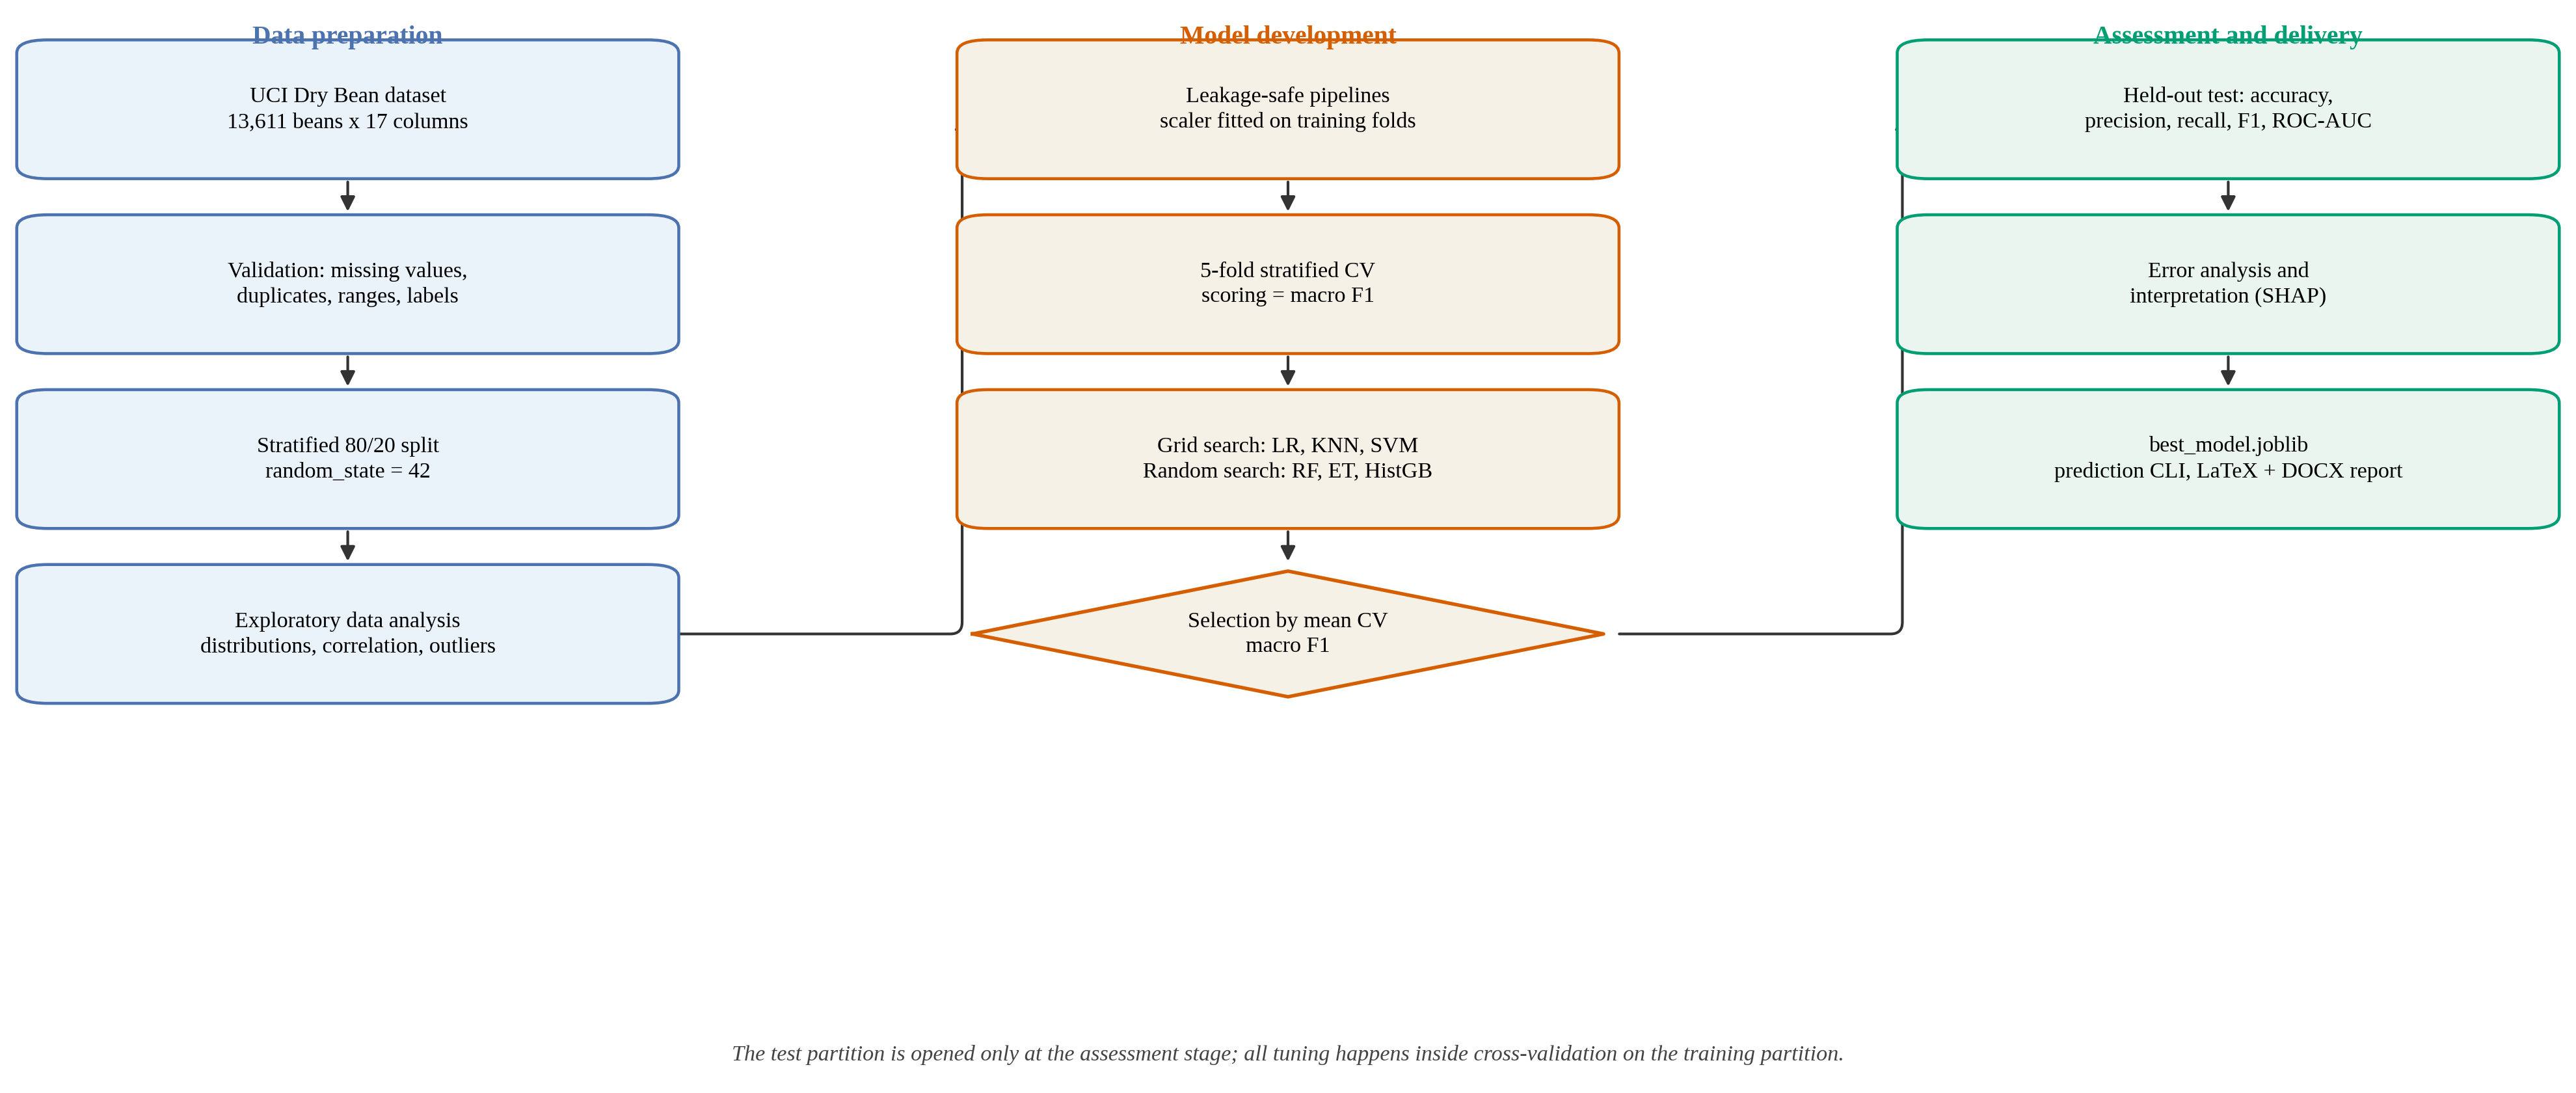
\includegraphics[width=\textwidth]{fig_5_1_workflow.png}
\caption{End-to-end workflow. Model selection happens entirely inside the training
partition; the test partition is opened once, at the assessment stage.}
\label{fig:workflow}
\end{figure}

\section{Algorithms Selected}

Six classifiers were chosen so that the comparison spans the four classical
inductive biases: a linear decision boundary, a local instance-based rule, a
maximum-margin boundary in a kernel-induced space, and randomised tree ensembles.
The sixth, histogram gradient boosting, is included because the case-study brief
allows it and because it represents the boosted-tree family that the reviewed
literature does not cover on this dataset.

\subsection{Logistic Regression}

Multinomial logistic regression models the posterior of class $k$ as
\begin{equation}
  P(y = k \mid \mathbf{x}) =
  \frac{\exp(\mathbf{w}_k^{\top}\mathbf{x} + b_k)}
       {\sum_{j=1}^{K}\exp(\mathbf{w}_j^{\top}\mathbf{x} + b_j)},
  \qquad k = 1,\dots,K,
  \label{eq:softmax}
\end{equation}
and is fitted by minimising the L2-regularised negative log-likelihood
\begin{equation}
  J(\mathbf{W}, \mathbf{b}) =
  -\frac{1}{N}\sum_{i=1}^{N}\log P(y_i \mid \mathbf{x}_i)
  + \frac{1}{2C}\sum_{k=1}^{K}\|\mathbf{w}_k\|_2^{2}.
  \label{eq:lr-objective}
\end{equation}
The parameter $C$ is the inverse regularisation strength: small $C$ shrinks the
coefficients towards zero, large $C$ allows them to grow and lets the model fit
the training data more closely. The model has $K(d+1) = 7 \times 17 = 119$
parameters, solved here with the L-BFGS quasi-Newton method.

Logistic regression is included as the linear baseline, not as a candidate for the
final model. Its decision boundaries are hyperplanes in the 16-dimensional input
space, so it can only separate classes that are linearly separable or nearly so.
The exploratory analysis in Chapter~3 already indicates that this is false for the
five overlapping varieties: Cali and Barbunya differ mainly in a ratio, and a
hyperplane through standardised coordinates cannot express that cleanly. The
baseline quantifies how much accuracy the nonlinear models actually add.

\subsection{k-Nearest Neighbours}

kNN assigns the majority label among the $k$ nearest training points,
\begin{equation}
  \hat{y}(\mathbf{x}) =
  \arg\max_{c}\ \sum_{i \in \mathcal{N}_k(\mathbf{x})} w_i\,
  \mathbf{1}[y_i = c],
  \label{eq:knn}
\end{equation}
where $\mathcal{N}_k(\mathbf{x})$ is the set of $k$ nearest neighbours under a
chosen metric and $w_i = 1$ for uniform voting or $w_i = 1/d(\mathbf{x},
\mathbf{x}_i)$ for distance weighting. Euclidean and Manhattan metrics are both
searched, with $k \in \{1,3,5,\dots,41\}$.

The method has no training phase and no parametric assumption, which makes it a
useful contrast: it can represent arbitrarily curved boundaries, but it does so
purely from local density. Two properties make it sensitive here. It is entirely
dependent on the metric, so unscaled features would reduce it to a nearest-
\texttt{Area} rule; standardisation is therefore mandatory. And in 16 dimensions
the ratio between the nearest and farthest neighbour distances shrinks, so
distances become less discriminative as the feature set grows, which is the
curse of dimensionality. With 10,888 training beans and seven classes the
prediction cost is also non-trivial, since every query compares against the whole
training set.

\subsection{Support Vector Machine with an RBF Kernel}

The SVM finds the maximum-margin separating hyperplane \cite{cortes1995}. In its soft-margin primal
form for a binary problem,
\begin{equation}
  \min_{\mathbf{w}, b, \boldsymbol{\xi}}\ \
  \frac{1}{2}\|\mathbf{w}\|^{2} + C\sum_{i=1}^{N}\xi_i
  \quad\text{subject to}\quad
  y_i\big(\mathbf{w}^{\top}\phi(\mathbf{x}_i) + b\big) \ge 1 - \xi_i,\ \
  \xi_i \ge 0,
  \label{eq:svm-primal}
\end{equation}
where $\phi$ maps the inputs into a higher-dimensional space, $\xi_i$ are slack
variables that permit margin violations and $C$ prices those violations. The dual
form depends on the data only through inner products, so replacing
$\phi(\mathbf{x}_i)^{\top}\phi(\mathbf{x}_j)$ by a kernel $K(\mathbf{x}_i,
\mathbf{x}_j)$ gives a nonlinear classifier without ever computing $\phi$
explicitly. The radial basis function kernel used here is
\begin{equation}
  K(\mathbf{x}, \mathbf{x}') =
  \exp\!\big(-\gamma\|\mathbf{x} - \mathbf{x}'\|^{2}\big),
  \label{eq:rbf}
\end{equation}
whose single parameter $\gamma$ sets the width of the influence of a training
point. The decision function is
$\hat{y}(\mathbf{x}) = \operatorname{sign}\big(\sum_i \alpha_i y_i
K(\mathbf{x}_i, \mathbf{x}) + b\big)$, and only the points with $\alpha_i > 0$,
the support vectors, contribute.

The two hyperparameters have opposite and interacting effects. Large $C$ penalises
margin violations heavily, producing a wiggly boundary that follows the training
data; small $C$ produces a smoother boundary that may underfit. Large $\gamma$
makes each training point influential only in a small neighbourhood, which again
overfits; small $\gamma$ makes the kernel almost linear. Because the effects
interact, both were searched jointly over a $4\times4$ grid rather than tuned one
at a time. The SVM is the primary candidate for this dataset because the class
boundaries are expected to be curved but not arbitrarily so: the EDA shows
compact, roughly ellipsoidal clusters, which is the geometry an RBF kernel
represents well.

One implementation detail matters for the results. The binary formulation above
does not extend directly to seven classes. scikit-learn's \texttt{SVC} uses the
one-versus-one scheme, training $\binom{7}{2} = 21$ binary classifiers and
deciding by a voting scheme, so the fitted model contains 21 margins rather than
one. The reported predictions are therefore the output of a pairwise voting
procedure, not of a single seven-way optimisation. Class probabilities, where
needed for the ROC curves, are obtained by Platt scaling \cite{platt1999}, which
fits a logistic model to the decision values using an internal cross-validation.

\subsection{Random Forest}

A random forest \cite{breiman2001} averages $T$ decision trees, each grown on a bootstrap sample of
the training data and, at every split, allowed to consider only a random subset of
$\lfloor\sqrt{d}\rfloor$ or $\lfloor 0.5d\rfloor$ features. Splits are chosen to
maximise the decrease in Gini impurity
\begin{equation}
  G(t) = 1 - \sum_{k=1}^{K} p_{k\mid t}^{2},
  \label{eq:gini}
\end{equation}
where $p_{k\mid t}$ is the proportion of class $k$ in node $t$. The prediction is
the majority vote of the $T$ trees.

The two sources of randomness decorrelate the trees, and averaging correlated
predictors with variance $\sigma^2$ and pairwise correlation $\rho$ gives an
ensemble variance of roughly
\begin{equation}
  \operatorname{Var}\!\left(\frac{1}{T}\sum_{t=1}^{T} h_t(\mathbf{x})\right)
  = \rho\sigma^{2} + \frac{1-\rho}{T}\sigma^{2},
  \label{eq:rf-variance}
\end{equation}
so the benefit comes from lowering $\rho$, not from adding trees indefinitely.
That is why the number of trees is a cost parameter rather than a tuning
parameter: increasing $T$ reduces the second term only, and the first term is
controlled by the feature subsampling. For this reason $T$ was fixed at 300 and
only the structural parameters were searched.

Random forests are included because they make no assumption about the shape of the
boundary, are invariant to monotone rescaling, and handle the redundant features
of Chapter~3 without difficulty: if two columns carry the same information, the
forest simply uses whichever is drawn at a given node. Their weakness is that
axis-aligned splits approximate diagonal or ratio-based boundaries only with many
small steps, which is exactly the geometry that separates Cali from Barbunya.

\subsection{Extra Trees}

Extremely randomised trees \cite{geurts2006} use the same ensemble structure but differ in one
respect: instead of searching for the best threshold at each node, a random
threshold is drawn for each candidate feature and the best of those random splits
is kept. The trees are therefore more strongly randomised and individually more
biased, but less correlated, which by Equation~\ref{eq:rf-variance} can reduce
ensemble variance. The method also trains faster, because no sorting of candidate
thresholds is required. The comparison between Random Forest and Extra Trees is
therefore a direct test of whether the extra randomisation helps on this feature
set, with everything else held constant.

\subsection{Histogram Gradient Boosting}

Gradient boosting fits trees sequentially, each one to the negative gradient of
the loss with respect to the current ensemble prediction. The histogram variant
discretises each feature into at most 255 bins, which makes split search
$O(N)$ per feature and allows deep ensembles to be trained quickly. The learning
rate, number of boosting rounds, leaf count, minimum leaf size and L2 penalty were
searched. Boosting is included as a sixth model because it often outperforms
bagging on tabular data with moderate sample size, and because including it makes
the comparison cover both ensemble strategies.

\section{Implementation Details}

The implementation is Python 3.12.13 with NumPy 2.3.4 \cite{harris2020},
pandas 2.3.3 \cite{mckinney2010}, scikit-learn 1.7.2 \cite{pedregosa2011},
SciPy 1.16.2 \cite{virtanen2020}, Matplotlib 3.10.7 \cite{hunter2007} and
seaborn 0.13.2 \cite{waskom2021}. All
experiments ran on a 12-core x86-64 desktop with 30~GB of RAM and no GPU; the
pipeline never uses one. The complete run, from download to the last SHAP plot,
takes \PipelineMinutes{} minutes.

Table~\ref{tab:modules} lists the modules and their responsibilities. Each module
is importable, has a \texttt{\_\_main\_\_} entry point where that makes sense, and
writes its outputs to a fixed directory, so any stage can be re-run alone.

\begin{table}[htbp]
\centering
\caption{Implementation modules}
\label{tab:modules}
\small
\begin{tabularx}{\textwidth}{@{}lX@{}}
\toprule
\textbf{Module} & \textbf{Responsibility} \\
\midrule
\texttt{config.py} & paths, random seed, feature order, colour palette, plot style \\
\texttt{data\_loader.py} & download, load, integrity validation, JSON report \\
\texttt{preprocessing.py} & stratified split, pipeline factory, split artefacts \\
\texttt{eda.py} & descriptive statistics and all Chapter 3 figures \\
\texttt{train.py} & model zoo, grid and random search, selection, ablations \\
\texttt{evaluate.py} & held-out metrics, confusion matrices, ROC, error analysis \\
\texttt{explainability.py} & impurity, permutation and SHAP importance \\
\texttt{predict.py} & command-line and programmatic prediction \\
\texttt{run\_pipeline.py} & orchestration of the six stages \\
\bottomrule
\end{tabularx}
\end{table}

Two implementation decisions affect the runtime and are worth recording. First,
parallelism is applied at the level of the cross-validation search: each candidate
configuration is evaluated in a separate process, which is the only effective
option for the SVM because the underlying libsvm solver is single-threaded. Nested
parallelism was deliberately avoided, since running a multi-threaded forest inside
a multi-process search oversubscribes the cores and makes the run slower.
Second, the search spaces were pruned of configurations that cannot change the
model. With 16 features, \texttt{max\_features="sqrt"}, \texttt{"log2"} and
\texttt{0.3} all select four features and are therefore the same estimator; only
\texttt{"sqrt"} and \texttt{0.5} are retained. Similarly,
\texttt{n\_estimators} is fixed rather than searched. Removing those redundant
candidates cut the Random Forest search from 296~s to 184~s without changing the
selected model.

The prediction interface is a single function, shown in
Listing~\ref{lst:predict}, wrapped by a command-line entry point that accepts
either a CSV of measurements or all 16 values as flags.

\begin{lstlisting}[style=pycode, caption={Programmatic prediction. The saved
pipeline carries its own scaler, so callers never see raw feature scaling.},
label={lst:predict}]
def predict_records(records, model=None):
    model = model or load_model()
    frame = pd.DataFrame(records)[FEATURES].astype(float)
    proba = probabilities(model, frame)
    classes = list(model.classes_)
    ranked = np.argsort(proba[0])[::-1]
    return classes[ranked[0]], proba[0][ranked[0]]
\end{lstlisting}

\section{Hyperparameter Settings}

Table~\ref{tab:search_space} records the search space of every model. Grid search
was used where the space is small and its structure is interpretable (logistic
regression, kNN, SVM); randomised search with 25 and 20 draws was used for the
ensembles, where the product of the individual grids would be in the thousands and
most of that volume is uninformative. Every search used the same stratified
five-fold splitter with a fixed seed, so candidate configurations within a model
are compared on identical folds.

\begin{table}[htbp]
\centering
\caption{Hyperparameter search spaces}
\label{tab:search_space}
\footnotesize
\begin{tabularx}{\textwidth}{@{}p{2.5cm}p{4.6cm}p{4.2cm}X@{}}
\toprule
\textbf{Model} & \textbf{Hyperparameter} & \textbf{Values} & \textbf{Method} \\
\midrule
Logistic Regression & \texttt{C} & 0.01, 0.1, 1, 10, 100 & Grid (5) \\
\addlinespace
KNN & \texttt{n\_neighbors} & 1, 3, 5, 7, 9, 11, 15, 21, 31, 41 & \multirow{3}{*}{Grid (40)} \\
 & \texttt{weights} & uniform, distance & \\
 & \texttt{metric} & euclidean, manhattan & \\
\addlinespace
RBF-SVM & \texttt{C} & 0.1, 1, 10, 100 & \multirow{2}{*}{Grid (16)} \\
 & \texttt{gamma} & scale, 0.001, 0.01, 0.1 & \\
\addlinespace
Random Forest & \texttt{max\_depth} & None, 20, 30, 40 & \multirow{5}{*}{Random (25)} \\
 & \texttt{min\_samples\_split} & 2, 5, 10 & \\
 & \texttt{min\_samples\_leaf} & 1, 2, 4 & \\
 & \texttt{max\_features} & sqrt, 0.5 & \\
 & \texttt{n\_estimators} & fixed at 300 & \\
\addlinespace
Extra Trees & \texttt{max\_depth} & None, 20, 30, 40 & \multirow{5}{*}{Random (25)} \\
 & \texttt{min\_samples\_split} & 2, 5, 10 & \\
 & \texttt{min\_samples\_leaf} & 1, 2, 4 & \\
 & \texttt{max\_features} & sqrt, 0.5 & \\
 & \texttt{n\_estimators} & fixed at 300 & \\
\addlinespace
Hist Gradient Boosting & \texttt{learning\_rate} & 0.05, 0.1, 0.2 & \multirow{5}{*}{Random (20)} \\
 & \texttt{max\_iter} & 200, 400, 600 & \\
 & \texttt{max\_leaf\_nodes} & 31, 63 & \\
 & \texttt{min\_samples\_leaf} & 20, 50 & \\
 & \texttt{l2\_regularization} & 0.0, 1.0 & \\
\bottomrule
\end{tabularx}
\end{table}

Table~\ref{tab:best_params} lists the configuration selected for each model.
Figure~\ref{fig:svmgrid} shows the full SVM surface. It is flat between $C = 1$
and $C = 100$ at $\gamma = 0.01$, which means that once the margin penalty is
large enough the additional capacity is unused: the classes are already almost
separable in the induced space. The two failure modes appear at the corners.
$C = 0.1$ with $\gamma = 0.001$ underfits, because the kernel is too wide and the
penalty too weak to place a boundary; $\gamma = 0.1$ degrades every value of $C$,
because each training point then influences only its immediate neighbourhood and
the margin fragments.

\begin{table}[htbp]
\centering
\footnotesize
\caption{Best configuration of every model, chosen by mean 5-fold CV macro F1}
\label{tab:best_params}
\begin{tabular}{p{0.26\textwidth}p{0.64\textwidth}}
\toprule
Model & Selected hyperparameters \\
\midrule
RBF-SVM & C = 100.0, gamma = 0.01 \\
Hist Gradient Boosting & min\_samples\_leaf = 20, max\_leaf\_nodes = 63, max\_iter = 400, learning\_rate = 0.1, l2\_regularization = 1.0 \\
K-Nearest Neighbours & metric = euclidean, n\_neighbors = 9, weights = distance \\
Random Forest & min\_samples\_split = 10, min\_samples\_leaf = 2, max\_features = 0.5, max\_depth = 30 \\
Logistic Regression & C = 100.0 \\
Extra Trees & min\_samples\_split = 10, min\_samples\_leaf = 2, max\_features = 0.5, max\_depth = 30 \\
\bottomrule
\end{tabular}
\end{table}


\begin{figure}[htbp]
\centering
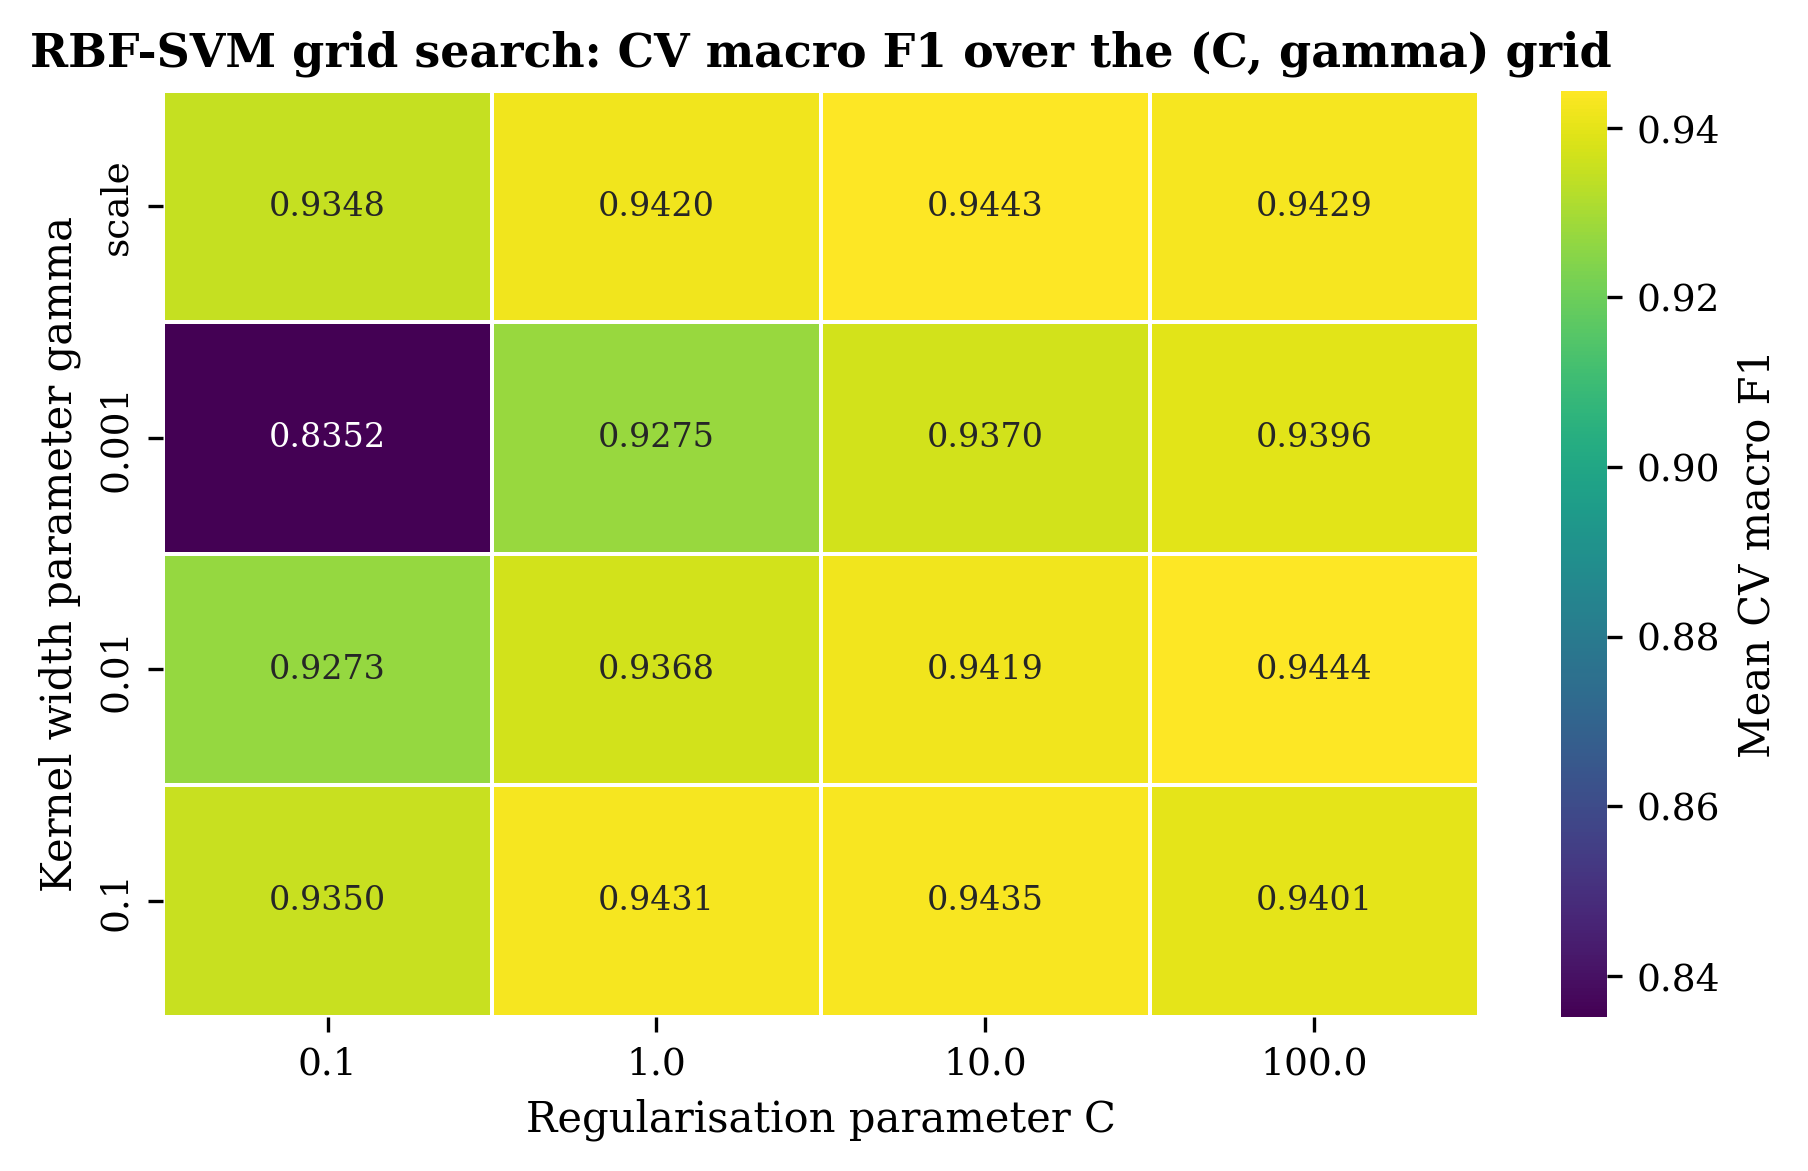
\includegraphics[width=0.60\textwidth]{fig_5_2_svm_grid_search.png}
\caption{Cross-validated macro F1 over the RBF-SVM $(\gamma, C)$ grid. The surface
is flat along the $C$ axis for $\gamma = 0.01$ and collapses at $\gamma = 0.1$.}
\label{fig:svmgrid}
\end{figure}
